\author{Antoine Cousson \\
Dylann Batisse \\
Margaux Schmied
}

\newcommand{\supervisorone}{Enrico Formenti}

\title{Neural Network and Learning \\Facial recognition: \\the mask/no mask case}
\date{2021/2022}

\documentclass[a4paper,12pt]{article}
\usepackage[left=30mm,top=30mm,right=30mm,bottom=30mm]{geometry}
\usepackage{etoolbox} %required for cover page
\usepackage{booktabs}
\usepackage[usestackEOL]{stackengine}
\usepackage[T1]{fontenc}
\usepackage[utf8]{inputenc}
\usepackage{bm}
\usepackage{graphicx}
\usepackage{subcaption}
\usepackage{amsmath}
\usepackage{amsfonts}
\usepackage{mathtools}
\usepackage{xcolor}
\usepackage{float}
\usepackage{hyperref}
\usepackage[capitalise]{cleveref}
\usepackage{enumitem,kantlipsum}
\usepackage{amssymb}
\usepackage[square,numbers,sort]{natbib}
\usepackage[ruled,vlined]{algorithm2e}
\usepackage{listings}
\usepackage{minted}
\usemintedstyle{emacs}
\usepackage{pgfplots}
\pgfplotsset{width=10cm,compat=1.9}
\setlength{\parindent}{0pt}
\usepackage[french]{babel}
\usepackage[T1]{fontenc}
\usepackage{listings}
\usepackage{color}
\usepackage{dirtree}
\usepackage{minted}

\definecolor{dkgreen}{rgb}{0,0.6,0}
\definecolor{gray}{rgb}{0.5,0.5,0.5}
\definecolor{mauve}{rgb}{0.58,0,0.82}

\bibliographystyle{unsrtnat}

\hypersetup{
    colorlinks,
    linkcolor={black},
    citecolor={blue!50!black},
    urlcolor={blue!80!black}
}

\linespread{1}

\newtheorem{theorem}{Theorem}[section]
\graphicspath{{figures/}}

\makeatletter
\def\maketitle{
  \begin{center}\leavevmode
       \normalfont
       
\includegraphics[width=0.6\columnwidth]{logo_master.png}
       \vskip 0.5cm
       \textsc{\large \department}\\
       \vskip 1.5cm
       \rule{\linewidth}{0.2 mm} \\
       {\large \exam}\\[1 cm]
       {\huge \bfseries \@title \par}
       \vspace{1cm}
	\rule{\linewidth}{0.2 mm} \\[1.5 cm]

	\begin{minipage}[t]{0.45\textwidth}
		\begin{flushleft} \large
			\emph{Auteurs:}\\
			\@author\\
		\end{flushleft}
	\end{minipage}
	\begin{minipage}[t]{0.45\textwidth}
	    \begin{flushright} \large
			\ifdefempty{\supervisortwo}{\emph{Supervisor:\\}}{\emph{Professeur:\\}}
			\supervisorone\\
			\ifdefempty{\supervisortwo}{}{\supervisortwo\\}
		\end{flushright}
	\end{minipage}
	\vfill
	{\Large \@date\par}
   \end{center}
   %\vfill
   %\null
   \cleardoublepage
  }
\makeatother

\begin{document}

\pagenumbering{gobble}

\maketitle

\tableofcontents

\newpage


\pagenumbering{arabic}

\section{Introduction}
L’objectif final de ce projet est de reconnaitre si les personnes sur des images portent un masque. Le projet se décompose en deux parties, la première est un logiciel permettant d’annoter des images. Les images annotées nous serviront ensuite pour entrainer le réseau de neurones dans la seconde partie.
Vous pouvez retrouver le travail de ces deux parties sur les deux repositories suivant : 
\begin{itemize}
    \item \href{https://github.com/MonsieurCo/facial-recognition}{Première Partie}
    \item \href{https://github.com/takitsu21/mask-no-mask-detection}{Seconde Partie}
\end{itemize}



\part{Logiciel d'annotation d'images}
\section{Objectif du logiciel}

Le but de la première partie est de réaliser un logiciel d’annotation d’images en python pour fournir un jeu de données à nôtre IA dans la seconde partie du projet.\\

Nous avons dû donner la possibilité à l'utilisateur d'encadrer une ou plusieurs parties de l'image puis de leur assigner une catégorie. Chaque cadre doit pouvoir être éditable, pour changer la catégorie ou supprimer le cadre. L’utilisateur doit pouvoir sauvegarder toutes ses annotations. En ce qui concerne les catégories il est nécessaire de pouvoir en importer, en ajouter ou en supprimer.

\section{Base de donnée}
Pour récolter les données nécessaires à l'entrainement de l'IA nous nous sommes rendu sur \href{https://www.kaggle.com/swann00/masque-vs-sans-masque}{kaggle.com} où nous avons recherché un jeu de données composé de différentes personnes. Nos critères étaient d'y trouver des personnes dans diverses situations, de différents âges, ethnies et en nombre varié pour avoir une diversité suffisante, afin d'éviter les problèmes liés à un jeu de données trop réduit. Cependant les images nous semblent petites, nous verrons dans la seconde partie du projet si elles conviennent bien à nos besoins.\\

Pour la partie annotation, nous avons enregistré pour chaque image dans un JSON, un identifiant unique, les coordonnées des zones annotées associées au titre d'une catégorie, sa taille ainsi que le chemin vers cette dernière. En revanche la sauvegarde n'est pas automatique, il faut enregistrer à la fin de chaque session d'annotation dans un fichier JSON.

\newpage
\section{Choix de conception}

\begin{description}
\item Méthodologie:
Pour mieux s'organiser au cours du projet nous avons utilisé l'outil de versioning git.
Cet outil nous a permis de travailler à plusieurs sur différentes branches en simultané et enfin de fusionner le tout pour avoir un produit tout le temps fonctionnel.

\item Technologies : \textbf{Python3.9.9}\\
Pour réaliser l'interface graphique de ce projet nous nous sommes plutôt rapprochés d'une librairie externe nommée Qt, développée en \textit{C++} qui selon nous est plus ergonomique que le GUI classique de Python \guillemotleft \textbf{tkinter}\guillemotright.\\
Qt est une librairie très puissante et moderne c'est pourquoi nous voulions en apprendre plus dessus.\\
Les différentes librairies utilisées au cours du projet sont :
    \begin{itemize}
        \item PySide6==6.2.1 (librairie Qt adapté pour python)
        \item Pillow==8.4.0 (redimensionner des images)
        \item Shapely==1.8.0 (intersections entre les rectangles)
    \end{itemize}
\end{description}



\section{Répartition des tâches}
Pour la répartition des tâches nous nous sommes organisés via GitHub et son système d'issues, mais aussi via Discord où nous recensions les bugs à réparer ainsi que les fonctionnalités à implémenter, nous passions par des phases de test où nous essayions de mettre le logiciel à l'épreuve pour détecter les bugs potentiels. \\

Antoine s'est occupé de l'import et de l'export des données et des catégories, Dylann de toute la gestion des zones d'annotations, leur chevauchement, leur affichage et Margaux de la gestion des catégories, l'ajout, la suppression et la modification.

\section{Comment utiliser}
NOTE: Pensez à mettre les droits d'exécution sur le fichier \textbf{build.sh} pour installer les dépendances et lancer l'application.

Pour lancer :
\begin{verbatim}
#!/bin/bash
chmod u+x build.sh
./build.sh
\end{verbatim}
\clearpage

\begin{itemize}
    \item Pour \textbf{ouvrir un fichier ou un dossier} via la menu-bar ou en effectuant un drag and drop sur la zone prévue à cet effet.
    \item Pour \textbf{ouvrir une image}, une fois le dossier ouvert, double-cliquez dessus et commencez à annoter.
    \item Pour \textbf{sélectionner une zone} vous pouvez appuyer sur clic gauche et étirer jusqu'à la taille souhaitée, la fenêtre de choix de categorie s'ouvre. Vous pouvez \textbf{séléctioner une categorie} et cliquer sur "Select category".
    \item Vous pouvez sélectionner plusieurs zones sur une même image.
    \item Pour \textbf{supprimer une annotation} faites clic droit sur la zone annotée de l'image.
    \item Pour \textbf{éditer une annotation} double-cliquez dessus, la fenêtre des choix de catégorie va apparaitre et vous pourrez éditer votre annotation.
    \item Pour \textbf{éditer une catégorie} double-cliquez dessus pour qu'elle devienne éditable, une fois la modification faite, appuyez sur "Change Category" pour valider le changement, qui se reportera dans le fichier JSON d'annotation.
    \item Pour \textbf{supprimer une categorie} selectionner là et cliquer sur "Delete category".
    \item Pour \textbf{ajouter  une categorie} écriver son nom dans la zone éditable en haut et cliquer sur "Ok".
    \item CTRL + S : Sauvegarder.
    \item CTRL + O : Ouvrir un fichier.
    \item CTRL + SHIFT + O : Ouvrir un dossier.
    \item CTRL + W : Quitter une image.
    \item CTRL + H : Ouvrir ce README.
\end{itemize}

\begin{center}
    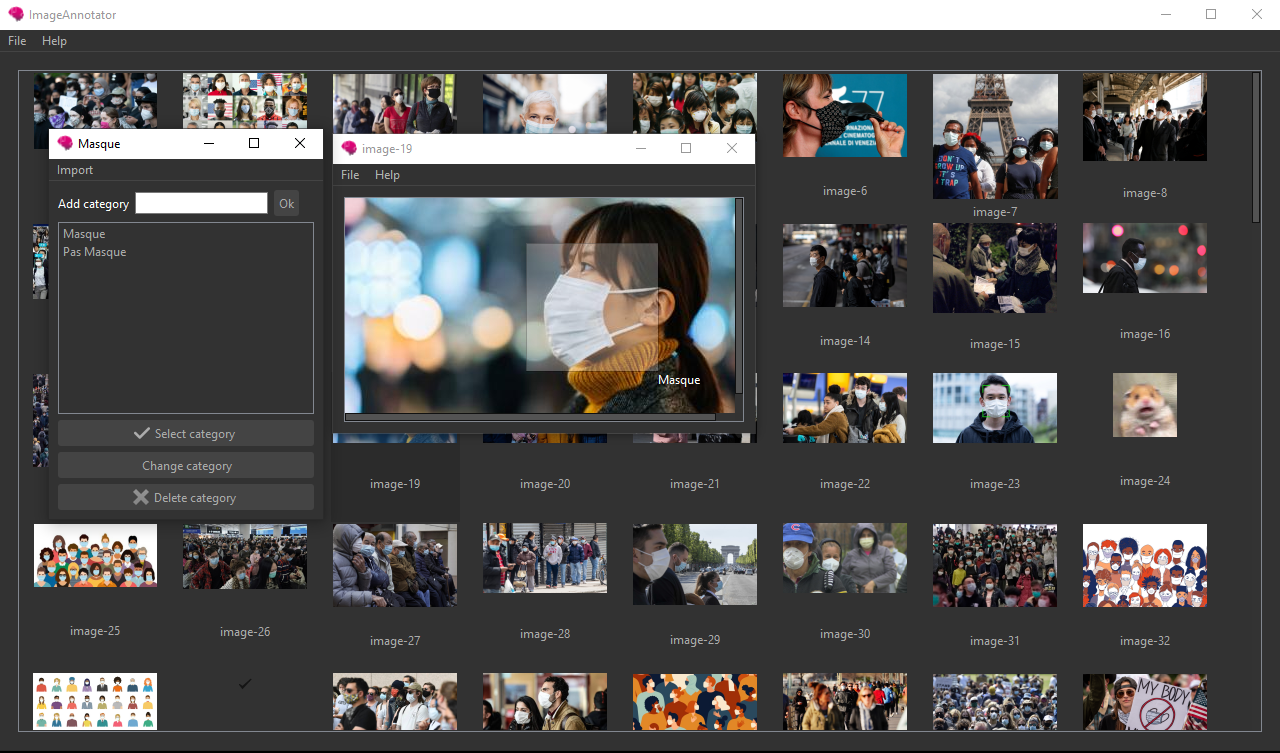
\includegraphics[scale=0.3]{resources/annotation.png}
    \captionof{figure}{Logiciel en action}
\end{center}


\section{Amélioration possible du logiciel}

Nous avons pensé à implémenter un système de Ctrl-Z Ctrl-Y à l'avenir sur l'édition des zones d'annotations, c'est une fonctionnalité qui paraît simple en apparence mais nous demande beaucoup de travail en arrière-plan, invisible pour l'utilisateur.
Nous avons testé le logiciel à la recherche de bug, ce qui a permis d'en régler plusieurs lors de cette période. Nous n'en avons plus trouvé après les corrections de ceux recensés. \\
Le projet étant très intéressant nous avons imaginé continuer le logiciel et peut-être faire en sorte d'annoter des vidéos pour que l'on puisse à partir d'une séquence obtenir une multitude d'images et entrainer l'IA sur celle-ci voir même sur des films.


\section{Conclusion du logiciel d'annotation}

Lors de cette première partie nous avons donc réalisé ce logiciel de façon à ce qu’il nous convienne pour travailler pour la seconde partie. Nous avons implémenté les fonctionnalités qui nous semblaient utiles, pour pouvoir annoter efficacement les images. En effet si nous avons un logiciel ergonomique, nous faciliterons la phase de création du jeu de données d'images, pour nourrir notre algorithme. \\

Cette partie nous a permis de prendre en main les librairies graphiques en python et de faire attention à l'efficacité du logiciel.
\newpage

\part{Detection du port du masque}

\section{Objectif de detection}

Le but de la deuxième partie est de détecter les visages sur des images. Puis de classer ces visages dans une catégorie \textbf{Masque} ou \textbf{Pas masque}.
Pour cela nous avons dû concevoir une base de données, sélectionner et entrainer un modèle, trouver les meilleurs paramètres pour ce dernier et afficher les résultats prédits.

\section{Choix de conception}

\subsection{Choix des outils}

\begin{itemize}
\item Technologies : \textbf{Python3.9.9}\\
Pour réaliser la seconde partie du projet nous avons utilisé les librairies suivantes:\\
    \begin{itemize}
        \item PySide6==6.2.2.1 (librairie Qt adapté pour python)
        \item Pillow==9.0.0 (redimensionner des images)
        \item tensorflow==2.7.0
        \item opencv-python==4.5.5.62
        \item tabulate==0.8.9
        \item tqdm==4.62.3 
        \item scikit-learn==1.0
        \item matplotlib==3.4.3
        \item numpy==1.22.0
    \end{itemize}
\end{itemize}

\subsection{Installation}

Vous pouvez utiliser le fichier \textbf{install.sh}

\begin{verbatim}
$ chmod u+x install.sh
$ ./install.sh
\end{verbatim}
soit

\begin{verbatim}
$ python3 -m pip install -r requirements.txt
\end{verbatim}


\section{Comment utiliser}

\subsection{Ligne de commande}

Commande d'aide : \\
\begin{verbatim}
$ python3 main.py -h

usage: main.py [-h] [-i IMG_PATH] [-tr TRAIN] [-mp MODEL_PATH] [-e EPOCHS] 
[-b BATCH_SIZE] [-w WORKERS] [-dir DIR_PREDICT_PATH]

Predict classes of an image

optional arguments:
  -h, --help            show this help message and exit
  -i IMG_PATH, --image IMG_PATH
                        Image path (default: None)
  -tr TRAIN, --train TRAIN
                        Train the model
  -mp MODEL_PATH, --model_path MODEL_PATH
                        Path to the model (default: model.h5)
  -e EPOCHS, --epochs EPOCHS
                        Epoch size (default: 25)
  -b BATCH_SIZE, --batch_size BATCH_SIZE
                        Batch size (default: 32)
  -w WORKERS, --workers WORKERS
                        Number of workers (default: 1, if > 1 activate multiprocessing)
  -dir DIR_PREDICT_PATH, --dir_predict_path DIR_PREDICT_PATH
                        Path to the directory with images
\end{verbatim}
\\
\textbf{Entrainer une IA :}

\begin{verbatim}
python3 main.py --train true -w 8 -mp "model.h5" -e 40 -b 40
\end{verbatim}

\textit{Entrainement de l'IA et utilisation de 8 workers avec 40 epochs et 40 batchs.
} \\

\textbf{Prédire une image :} 

\begin{verbatim}
python3.9 main.py -i img_tests/test.png -w 8 -mp "model.h5"
\end{verbatim}

\textit{Prédiction de l'image test.png et utilisation de 8 workers avec le modèle "model.h5"}

\begin{center}
    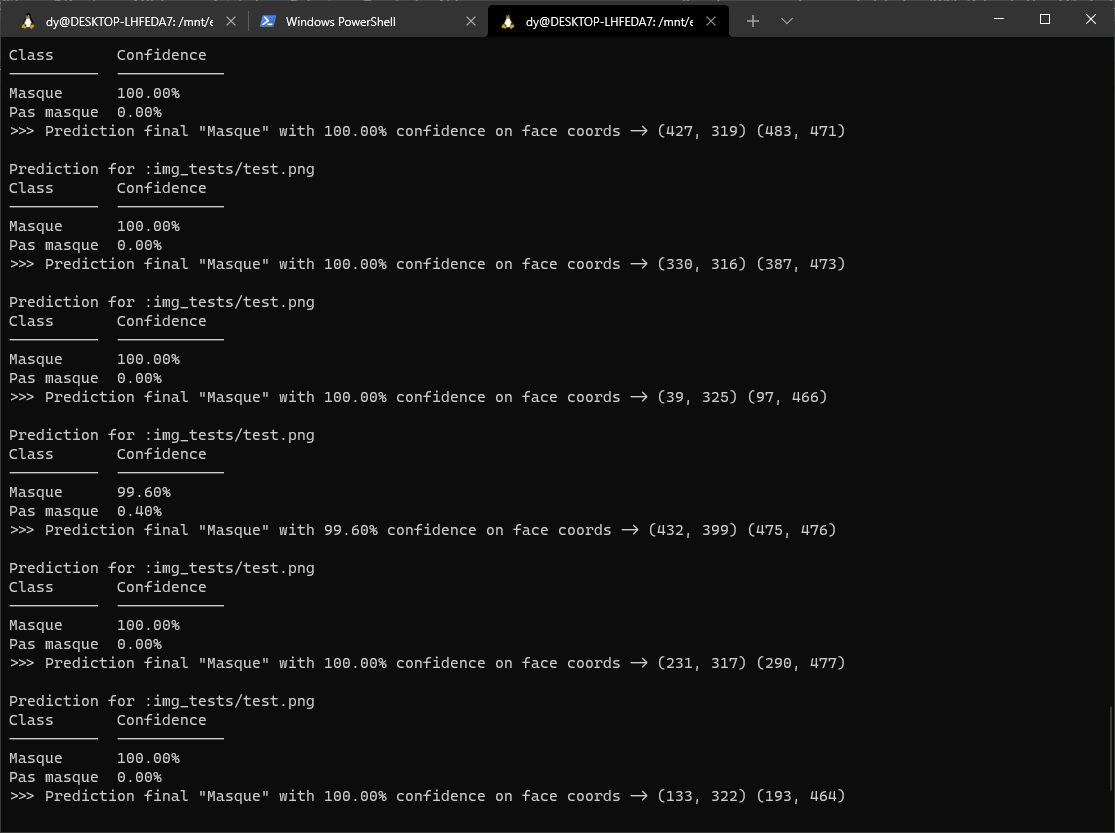
\includegraphics[scale=0.5]{resources/command_line_prediction.png}
    \captionof{figure}{Prédiction en ligne de commande sur une image}
\end{center}

\clearpage


\subsection{Interface graphique}

\begin{verbatim}
    python3 app.py
\end{verbatim}
\begin{itemize}
    \item Pour \textbf{ouvrir un fichier ou un dossier} via la menu-bar ou en effectuant un drag and drop sur la zone prévue à cet effet.
    \item Pour \textbf{ouvrir une image}, une fois le dossier ouvert, double-cliquez dessus et l'image avec les predictions va s'ouvrir.
\end{itemize}

\begin{center}
    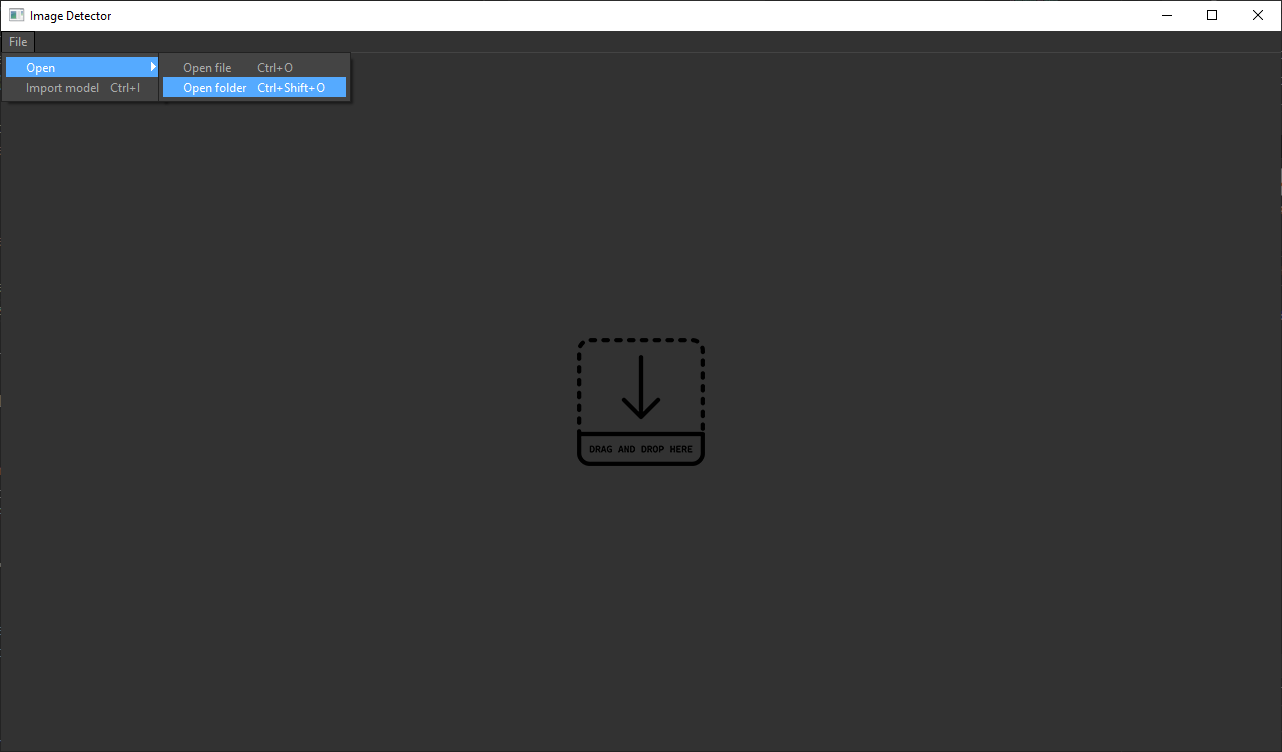
\includegraphics[scale=0.4]{resources/software_import_folder.png}
    \captionof{figure}{Importer un répertoire d'images}
\end{center}

\begin{center}
    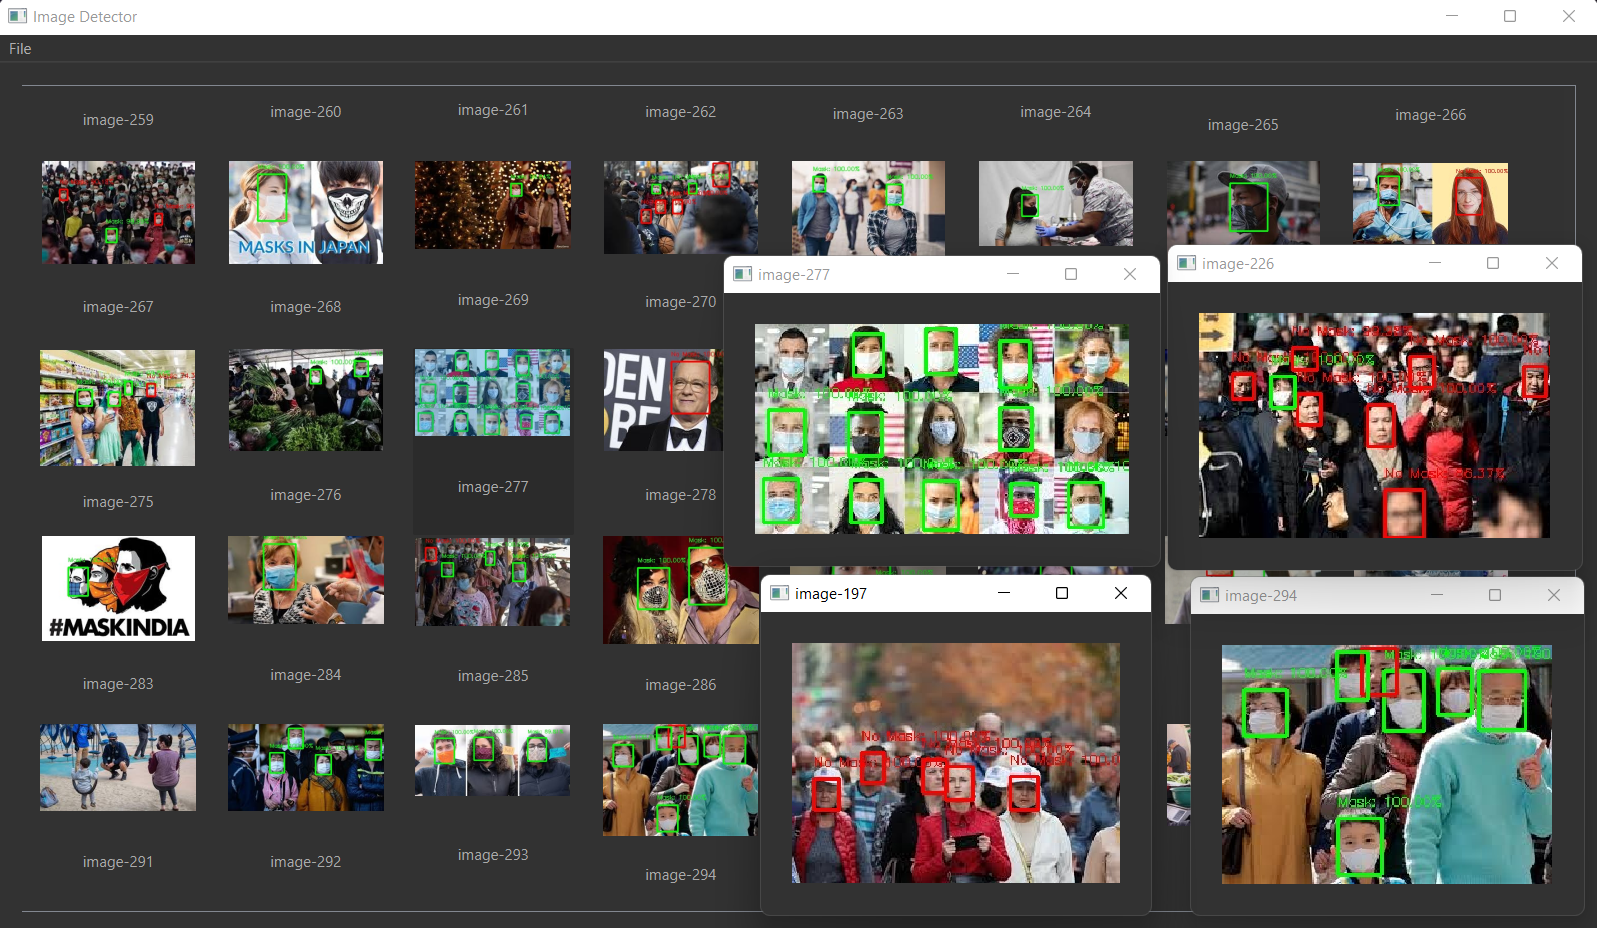
\includegraphics[scale=0.4]{resources/software_predict_folder.png}
    \captionof{figure}{Prédiction du répertoire d'images}
\end{center}
\begin{itemize}
    \item CTRL + i : Importer un modèle.
    \item CTRL + o : Ouvrir un fichier.
    \item CTRL + SHIFT + O : Ouvrir un dossier.
\end{itemize}


\section{Jeu de Données}

Afin d'entrainer le réseau de neurones nous avons préparé un jeu de données en utilisant le logiciel réalisé dans la première partie. Nous sommes partis d'une banque de 200 images disponibles sur \href{https://www.kaggle.com/swann00/masque-vs-sans-masque}{kaggle.com}, la même que dans la première partie.
Nous avons ensuite annoté les images en indiquant la présence ou l'absence de masque sur un visage.
Une fois nos images annotées nous exportons ces informations sous un format JSON que nous couplons aux images mises au bon format (\textbf{.png}).\\
Par la suite nous recadrons les images en fonction des zones annotées et les plaçons dans un dossier portant le nom de leur catégorie, via un programme de compréhension de notre ficher d'annotations que nous avons réalisé.  \\
Après quelques tests les résultats étaient présents mais pas assez précis. \\
Pour que notre modèle ait plus de diversité nous nous sommes basés sur un autre jeu de données d'environ 2000 images pour détecter les masques et 2000 images sans masques, ce dataset est disponible sur \href{https://github.com/balajisrinivas/Face-Mask-Detection/tree/master/dataset}{GitHub}.

Une fois cette étape finie nous pouvons construire un objet en python nommé \textit{ImageDataGenerator} nous permettant de normaliser les images recadrées (même taille, même encodage couleur, ...). Cela nous permet aussi de faire de l'augmentation de données, en produisant des rotations ou des changements de couleurs pour éviter les problèmes liés au surapprentissage (overfitting). \\

\textbf{Arboresence du dossier utilisé pour le jeu de données.}
\dirtree{%
.1 dataset.
.2 Masque.
.2 Pas Masque.
}

\section{Implémentation et choix du modèle}

Nous avons décidé de nous appuyer sur un modèle préexistant de l'api \textbf{Keras} nommée \textbf{ResNet50V2} qui nous fournit 50 layers optimisés pour pouvoir entrainer nos IA. \\
Il en existe d'autres mais nous n'avons pas pu tous les tester par manque de temps et nous avons rapidement eu des résultats convenables avec ce genre de modèle.
En effet entrainer un modèle est une tâche longue, ce qui nous a ralenti dans notre recherche d'un modèle adapté.

\clearpage
\section{Test du modèle}

Nous avons vu qu’il était important de faire varier les paramètres dans le but de faire augmenter la précision (accuracy) et diminuer le taux d’erreur.
Nous avons donc fait varier les paramètres \textbf{epochs} et \textbf{batch\_size} ainsi que les \textbf{layouts}.\\

L'\textit{epoch} est une itération complète sur des échantillons. Le nombre d'epochs correspond au nombre de fois où l'algorithme va s'exécuter. Le nombre d'epoch affecte le résultat de l'étape d'apprentissage.\\

La \textit{Batch Size} définit le nombre d'échantillons d'images qui seront introduits dans chaque itération du modèle. la Batch\_size est l'optimisation du poid du modèle, c'est à dire le nombre d'images effectuées en une étape de l'epoch. Si la Batch\_size est égale à 3, le modèle entrera 3 exemples d'images et seulement après ces 3 entrées, il mettra à jour les poids (weigths).\\


La \textit{loss} est une valeur qui représente la somme des erreurs dans notre modèle. elle mesure comment se porte notre modèle. Si les erreurs sont élevées, la Loss sera élevée, ce qui signifie que le modèle ne fait pas du bon travail. Sinon, plus la valeur est basse, mieux notre modèle fonctionne.\\

L'\textit{accuracy} mesure à quel point notre modèle prédit bien en comparant les prédictions du modèle avec les vraies valeurs.

\subsection{Epochs}
\begin{center}
    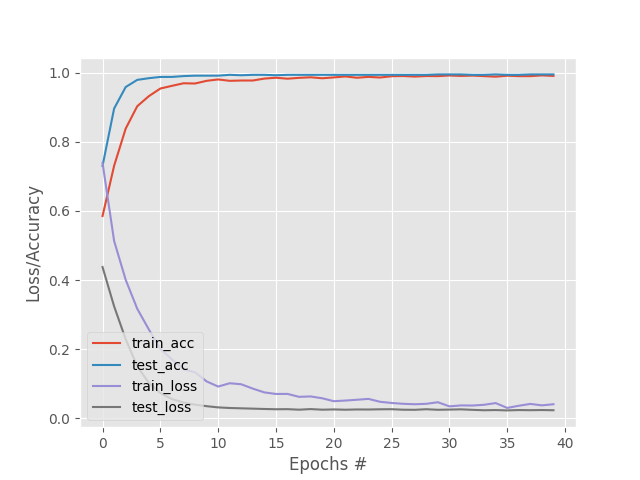
\includegraphics[scale=0.59]{resources/loss-accuracy.png}
    \captionof{figure}{Accuracy et loss en fonction des epochs}
\end{center}

Lorsque nous avons fait varier les epochs nous avons choisi de fixer la batch\_size arbitrairement à 40. On peut voir ici qu’à partir de 5 epochs l’accuraccy n’augmente plus de manière significative tandis que la loss diminue encore. Entre 30 et 40 la loss ne diminue quasiment plus. Nous avons donc choisi de garder \textbf{epochs = 40}.\\

\subsection{Batch size}

\begin{figure}[H]
  \centering
  \begin{subfigure}[b]{0.4\linewidth}
    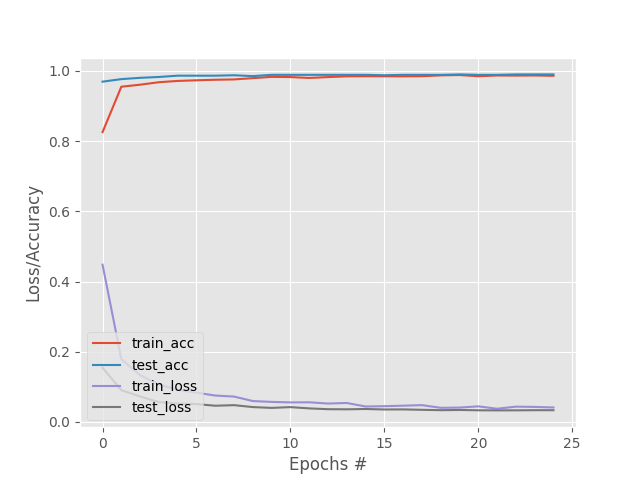
\includegraphics[width=\linewidth]{resources/loss-accuracy-25-1.png}
    \caption{Accuracy et loss avec une taille de batch de 1}
  \end{subfigure}
  \begin{subfigure}[b]{0.4\linewidth}
    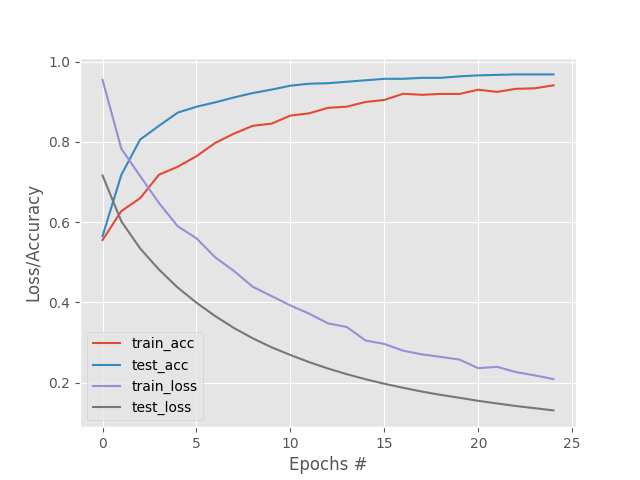
\includegraphics[width=\linewidth]{resources/loss-accuracy-25-129.png}
    \caption{Accuracy et loss avec une taille de batch de 129}
  \end{subfigure}
  \begin{subfigure}[b]{0.4\linewidth}
    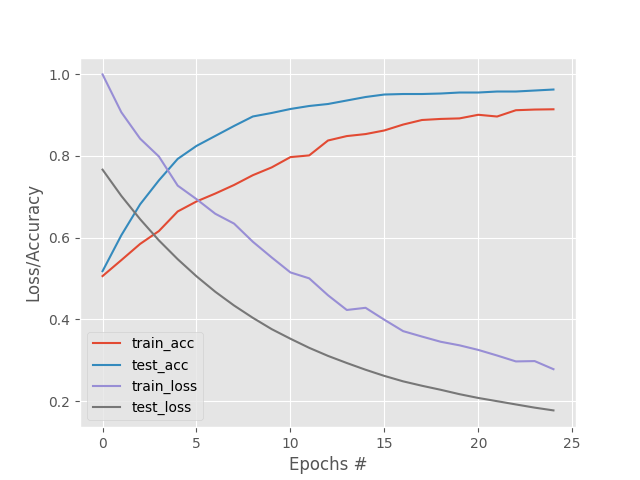
\includegraphics[width=\linewidth]{resources/loss-accuracy-25-257.png}
    \caption{Accuracy et loss avec une taille de batch de 257}
  \end{subfigure}
  \caption{Tests de la variation du batch size de 1 à 257}
  \label{fig:coffee}
\end{figure}

On peut voir dans les graphiques ci-dessus qu’avec l’augmentation des batch\_size l’accuracy augmente plus doucement. Plus la batch\_size est grosse plus le nombre d'epochs doit être grand. Il nous faut une batch\_size relativement élevé pour pouvoir reconnaitre une grande variété d’images. 

\clearpage
\subsection{Layers}

En entrée nous avons utilisé le modèle énnoncé précedemment le modèle \textbf{ResNet50V2}, nous nous sommes appuyés ensuite sur un type de modèle \textbf{CNN} (Convolution Neural Network) spécialisé dans la vision par ordinateur pour la classification d'images. \\

Un \textbf{CNN} est << \textit{un type de réseau de neurones artificiels acycliques (feed-forward), dans lequel le motif de connexion entre les neurones est inspiré par le cortex visuel des animaux. Les neurones de cette région du cerveau sont arrangés de sorte qu'ils correspondent à des régions qui se chevauchent lors du pavage du champ visuel. Leur fonctionnement est inspiré par les processus biologiques, ils consistent en un empilage multicouche de perceptrons, dont le but est de prétraiter de petites quantités d'informations. Les réseaux neuronaux convolutifs ont de larges applications dans la reconnaissance d'image et vidéo, les systèmes de recommandation et le traitement du langage naturel.} >> \\d'après \textbf{Wikipedia.} 


\begin{center}
    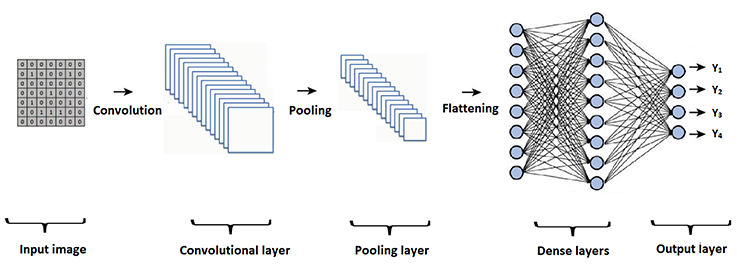
\includegraphics[scale=0.6]{resources/cnn.png}
    \captionof{figure}{Modèle CNN}
\end{center}

\section{Détection des visages}
Pour détecter les visages sur une image pour ensuite les analyser avec notre modèle, nous nous sommes servis d'un modèle de détection de visages éxistant via l'api \textbf{\href{https://fileinfo.com/extension/caffemodel}{caffemodel}} combiné à OpenCV qui nous permet d'utiliser des modèles de DeepLearning pour cibler les zones que nous analysons avec notre modèle.
Une fois la classification de la tranche de l'image faite, nous encadrons le visage et mettons une étiquette de la classe estimée.

\clearpage
\section{Problèmes rencontrés}

Une fois le modèle trouvé nous avons voulu essayer de classifier les masques FFP2, en tissus et chirurgicaux. Pour cela nous avons complété notre base de données avec plusieurs autres trouvées sur internet ainsi que des images récoltées à la main. Malheureusement cela n’a pas fonctionné. Nous soupçonnons que cela est dû à notre base de données peut-être trop petite ou de mauvaise qualité.


\section{Exemples}
Voici quelques exemples de la détection sur certaines images:\\


\begin{figure}[H]
  \centering
  \begin{subfigure}[b]{0.4\linewidth}
    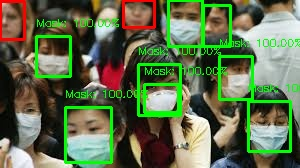
\includegraphics[width=\linewidth]{resources/images149-37.jpg}
  \end{subfigure}
  \begin{subfigure}[b]{0.34\linewidth}
    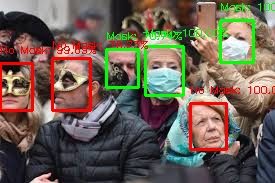
\includegraphics[width=\linewidth]{resources/images218-93.jpg}
  \end{subfigure}
  
  \begin{subfigure}[b]{0.4\linewidth}
    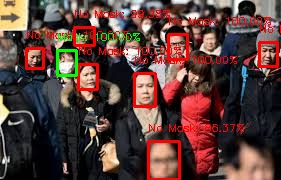
\includegraphics[width=\linewidth]{resources/images359-223.jpg}
  \end{subfigure}
  \label{fig:coffee}
   \begin{subfigure}[b]{0.35\linewidth}
    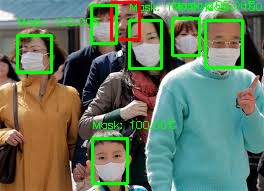
\includegraphics[width=\linewidth]{resources/images435-291.jpg}
  \end{subfigure}
\end{figure}


\section{Répartition des tâches}

Lors de cette partie nous avons eu plus de mal à découper le travail en tâches distinctes, nous avons donc codé en simultané via la fonction \textbf{liveshare} de \textbf{Visual Studio Code}. Nous avons effectué des recherches et testé des modèles. 
Avant de commencer le travail de programmation nous avons fait des sessions d'annotations d'images via notre logiciel.
Nous avons recherché des jeux de données, téléchargé des images, cela a été une partie non négligeable de notre travail.


\section{Améliorations possible du logiciel}
En terme d'améliorations, nous avons pensé essayer plusieurs modèles et les entrainer sur une longue période avec un jeu de données plus conséquent.
Nous pourrions aussi extraire d'un flux vidéo, une séquence d'images et appliquer notre modèle en temps réel sur le retour d'image, pour observer la détection, à partir d'une caméra.

\section{Conclusion}
Ce projet nous a permis de nous rendre compte de la puissance des réseaux de neurones et de la phase d'entrainement souvent cachée. \\
Nous nous sommes rendus compte qu'entrainer une IA était un processus lourd pour l'ordinateur, génerer une base de données en utilisant le logiciel d'annotations était fastidieu, mais une fois tout cela fait, c'est avec plaisir que nous avons pu observer le fonctionnement de notre IA.
Nous avons vu plusieurs manières de réaliser un modèle de classification et de détection mais aussi de l'entrainer ou même de construire le jeu de données.


\end{document}
